% Motivation - Description of PoS based system that motivates the design of a new solution. Specify the requirements on why PoS is not suitable in its current form and give motivation behind the solution architecture. 
% Chapter Template

\chapter{Motivation} % Main chapter title

\label{Chapter 2} % Change X to a consecutive number; for referencing this chapter elsewhere, use \ref{ChapterX}

\lhead{Chapter 2. \emph{Motivation}} % Change X to a consecutive number; this is for the header on each page - perhaps a shortened title

%----------------------------------------------------------------------------------------
%	SECTION 1
%---------------------------------------------------------------------------------------
\section{State Machine Replication}

In computer science, state machine replication or state machine approach is a general method for implementing a fault-tolerant service by replicating servers and coordinating client interactions with server replicas.


Blockchain systems are an example of such a system where a ledger of committed transactions acts as a common state between the replicas. These replicas are also known as miners. In a blockchain system, a leader is chosen to commit the new block to the ledger, and the commit is successful only when a consensus is reached on it. This consensus can be reached via two methods, Proof of Work based consensus or Proof of Stake based consensus.

% \section{Types of faults}

% \subsection{Crash Faults}

% A replica is said to be crash-faulty if it stops all computation and communication.

% \subsection{Byzantine Faults}

% A replica is said to be Byzantine or non-crash faulty if it acts arbitrarily, but cannot break cryptographic primitives we use (crypto- graphic hashes, MACs, message digests and digital signatures).

% \subsection{Network Faults}

% A network fault is defined as the inability of some correct replicas to communicate with each other in a timely manner, that is, when a message exchanged between two correct replicas cannot be delivered and processed within delay $\Delta$, known to all replicas.

\section{Proof Of Work based consensus}

In Proof of Work based consensus, the miners compete against each other to complete transactions on the network and get rewarded. The miners are required to solve a hard problem (Eg : Finding a number which when concatenated with the current block of transactions produces a hash which is less than a given number). Whichever miner solves the problem first becomes the leader for the current round and the number acts as his proof of work. The miner then gets to commit the next block to the ledger. To take over the system, an adversary needs to own more than half of the computation power in the network. This consensus system though secured has certain drawbacks. 
\begin{enumerate}
  \item To make sure that all the miners are updated with the current ledger and to generate the consensus for the next block, it is important for the system to have a minimum amount of delay between commitment of two consecutive blocks. And, as the number of miners grow, this delay increases and hence the latency increases too.
  \item As the number of miners increase in the network, the computation power of the network increases. And hence, the problem has to made harder and harder to solve to match with the delay required to for all miners to be in sync.
  \item As all the miners are trying to solve the same problem and only one comes on top as the winner. A lot of computational power is wasted in doing redundant work.
  \item Miners are also given transaction fees to incentivise them to compete against each other and use the computation power. And, this fees varies over time as the number of validators increase and value of the currency increases.
  \item The blockchain can only support finite number of transactions because as the number of nodes increase, you can only make the problem finitely much harder.
\end{enumerate}

Due to these drawbacks, the blockchain systems today are now adopting Proof of stake consensus protocols.

\section{Proof Of Stake based Consensus}

In a proof of stake system, the creator of the next block is determined by a randomized system that is, in part, dictated by how much of that cryptocurrency a user is holding or, in some cases, how long they have been holding that particular currency. Instead of computational power, as is the case in proof of work, the probability of creating a block and receiving the associated rewards is proportional to a user’s holding of the underlining token or cryptocurrency on the network. Eg : If a set of potential validators was made up of Adam, who is holding 40 tokens, Fil with 30, Tomek with 20 and Daniel with 10, there will be a 40\% chance of Adam being chosen to validate the block and Daniel 10\%, with Tomek and Fil on 20\% and 30\% respectively.

The randomization in a proof of stake system prevents centralization, otherwise the richest individual in the system would always be creating the next block and consistently increasing their wealth and as a result their control of the system. The main advantage of proof of stake, over a system such as proof of work, is that it uses considerably less energy and as a result is more cost effective. It is well documented that each Bitcoin transaction, which uses a proof of work system, can require as much electricity as an average Dutch household does in two weeks. This is both ineffective and unsustainable.

So, in total Proof of Stake consensus has following major benefits over Proof of Work consensus :

\begin{enumerate}
    \item It requires far less electricity to work as miners now don't need to waste computation power in doing redundant work of solving a hard problem.
    \item As the proof of stake system is so much more cost effective there is less of a need to release too many new coins as a means of incentivizing miners to maintain the network. This helps to keep the price of a particular coin more stable.
    \item The number of transactions that can be supported now is not finite, as now the miners don't have to solve a hard problem for proof of work
    \item Every node doesn't need to participate now in the validation. Only specially designated nodes participate in the consensus protocol.
    \item As the requirement of proof of work is removed, and the system is validated by a finite set of nodes, the system can work faster giving rise to higher throughputs and lower latencies. 
\end{enumerate}

\section{Drawbacks of POS consensus}

Even though the POS consensus has so many benefits, it has some of its drawbacks too. Following are some of them :

\begin{enumerate}
    \item The conventional POS systems are not as open as POW systems, one needs permission of the present member of the system to become part of the system or leave the system altogether
    \item The performance and trustworthiness of the system is largely affected by the number of validators present in the system. As the number of validators increase, trustworthiness of the system increases but the performance of the system goes down. POW systems have lower latencies but they maintain an average. Another reason why POS systems are designed to be closed.
    \item POS systems have geographical scalability issues. As the hops between the nodes increase, the performance of the system goes down. This happens because POS systems try to perform as better as possible but as the distance increases, it takes more time to form the consensus.
\end{enumerate}
Through this project, we are trying to tackle the first two issues of the Proof of Stake blockchain systems. In simple terms, our objective is to determine what's the correct number of validators in the system using market dynamics.

% \paragraph{Literature Survey}

% This is a sample. Write about referred papers. Cite like this \citep{nip2010cyclic}. Another example would be this \citep{nip2010extremely}. More citations like this \citep{bird2004evaluating}, \citep {tremblay2003seismic} and \citep {alhamaydeh2016key}.

% \paragraph{Research gaps}
% Typically include research gaps for your study. 
% \paragraph{Objective}
% Similarly objectives of study. 
% \paragraph{Scope}
% Define scope of study. 
% \paragraph{An algorithm}
% How you could refer to figures: This is an example. (Refer \ref{fig5}). You can add equations like this Eq. (\ref{eq1})
% \begin{equation}
% \label{eq1}
%   SDR = sd(T) - \sum_{i}\frac{{T}_{i}}{|T|}\times sd({T}_{i})
% \end{equation}

% \begin{figure}[]
% \centering
% 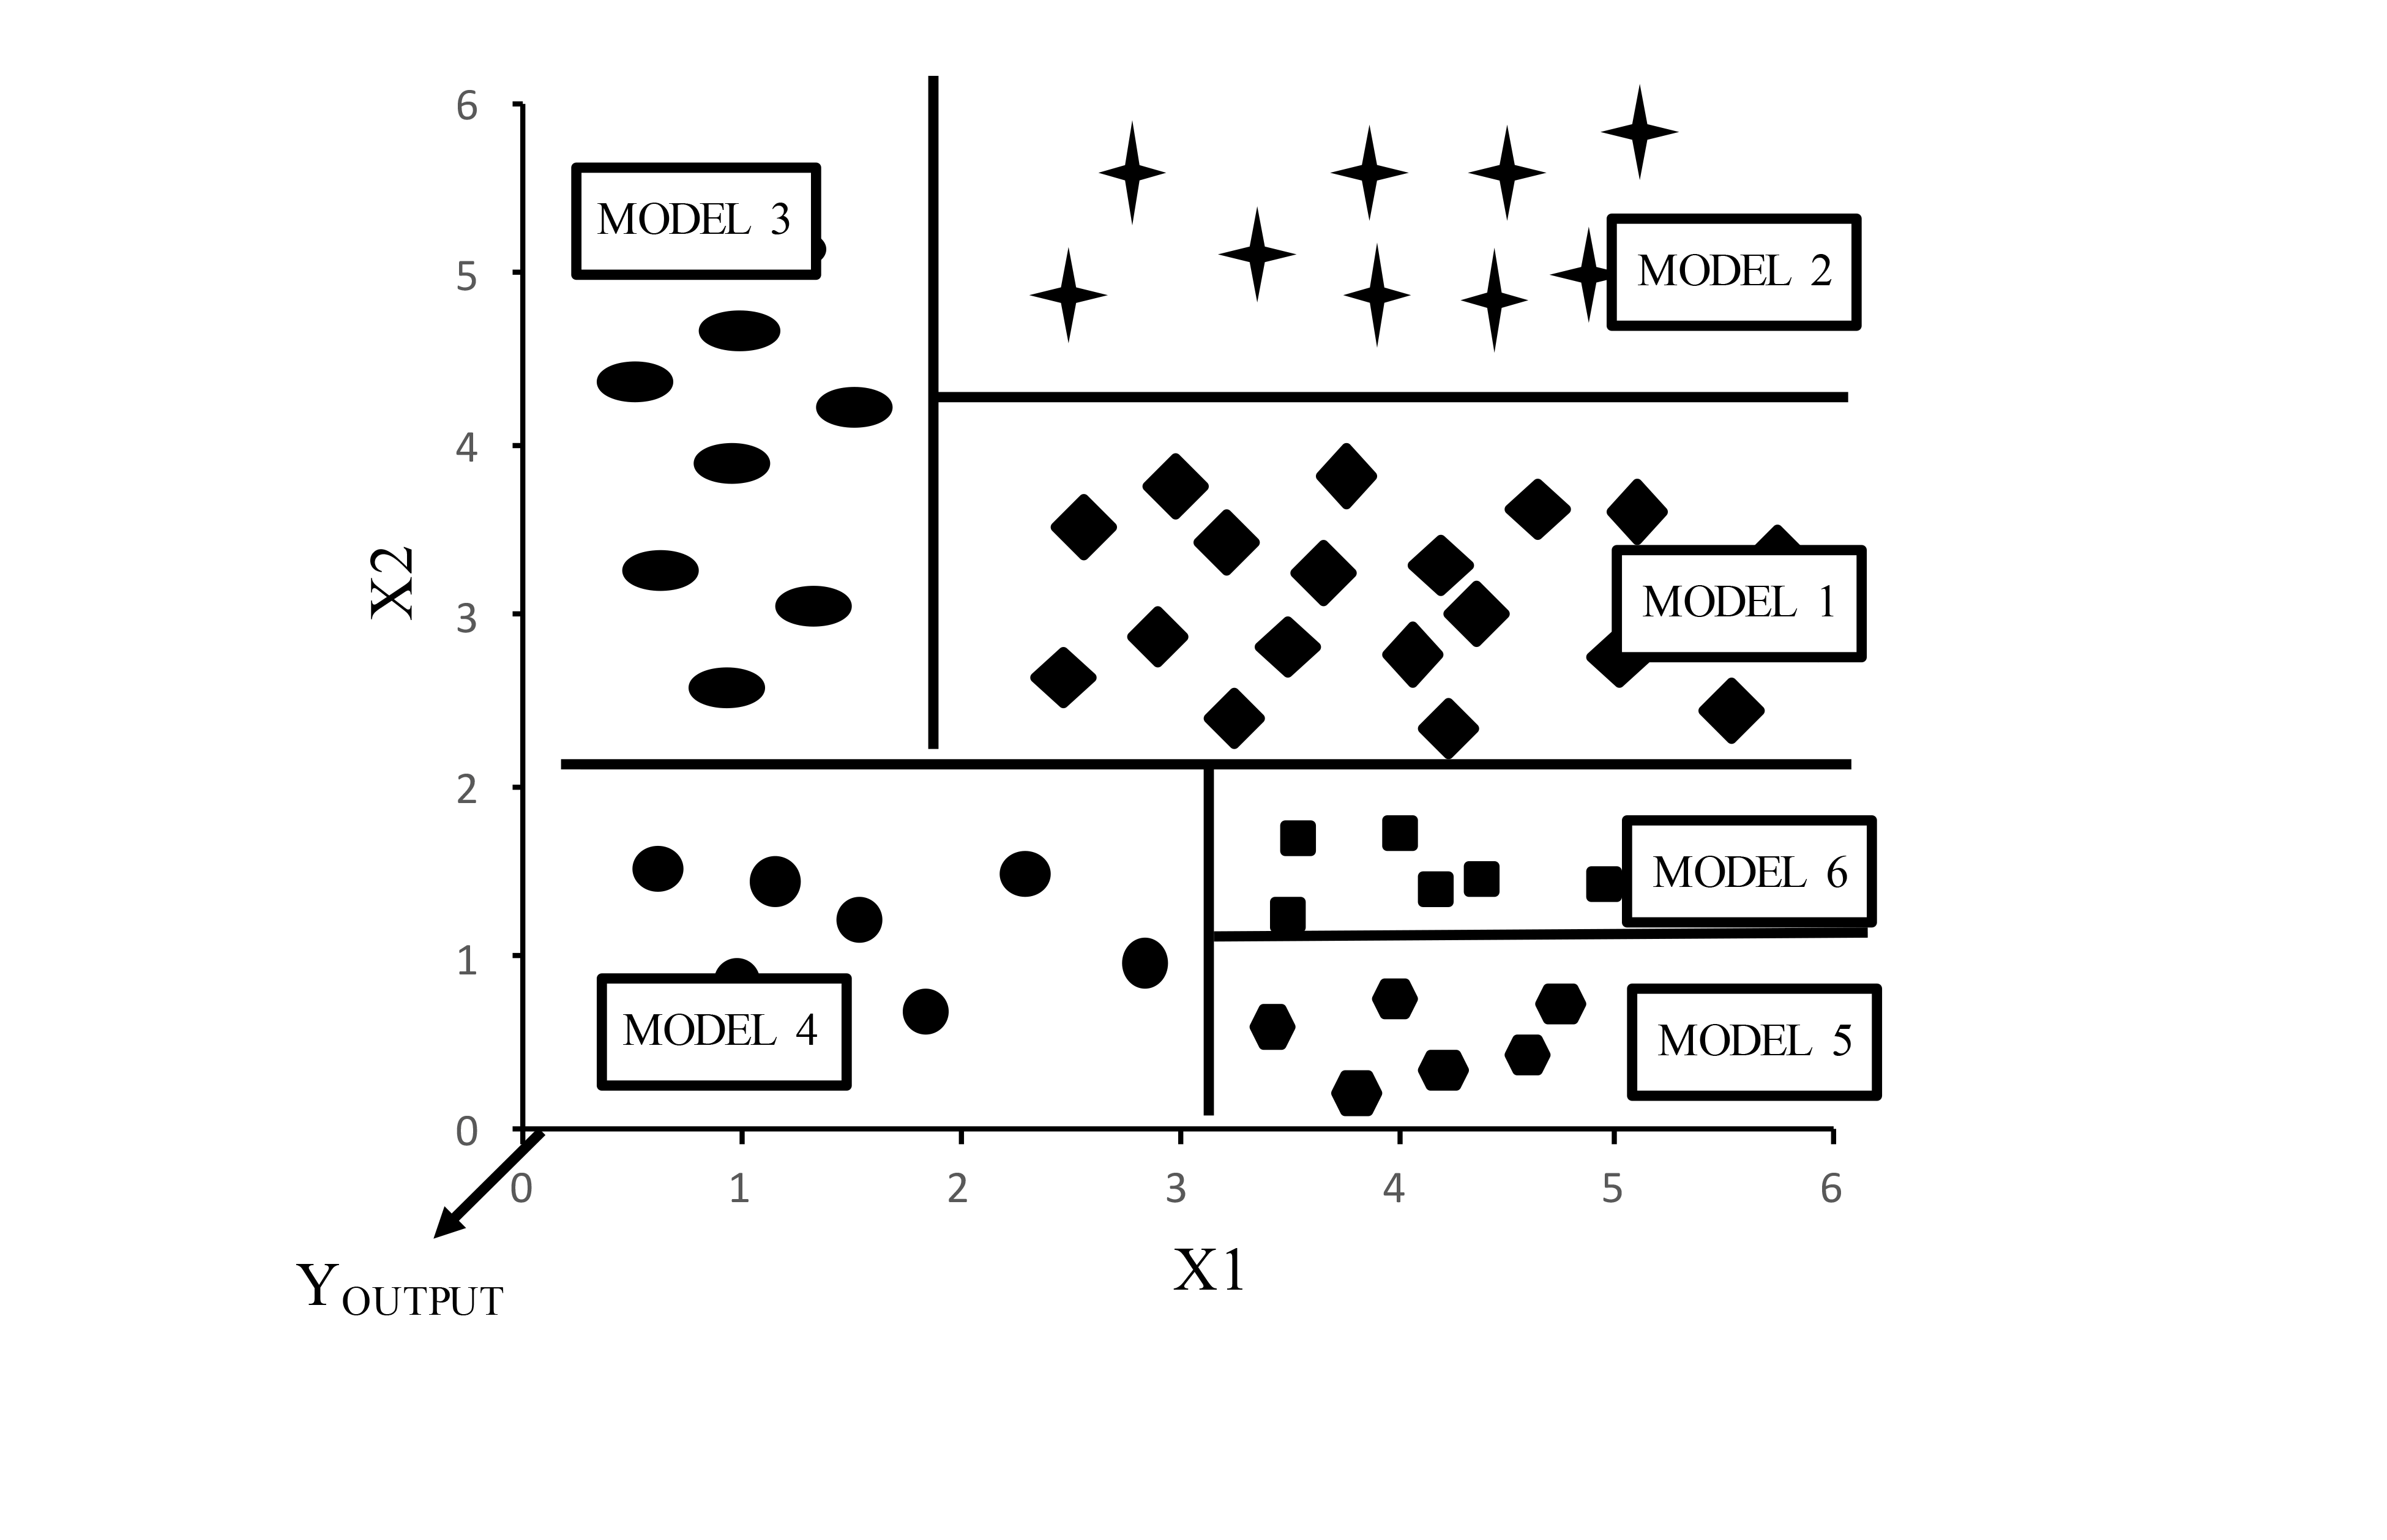
\includegraphics[height=7cm]{splits.png}
% \caption{Splitting of the input space (X1 x X2) by M5' model tree algorithm}
% \label{fig5}
% \end{figure}

% \section{Adding another section}
% You can show a lot of figures together like these Figures \ref{fig61}, \ref{fig62}, \ref{fig63} below.
% \begin{figure} [!htbp]
% \centering    
% \subfigure[Caption1]{\label{fig61}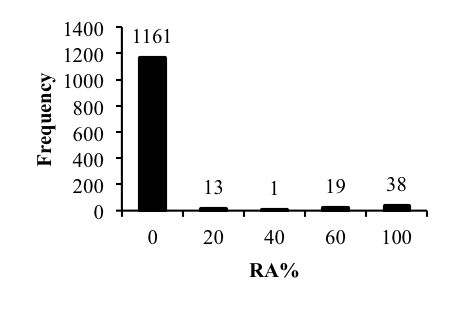
\includegraphics[width=42mm]{data1.png}}
% \subfigure[Caption2]{\label{fig62}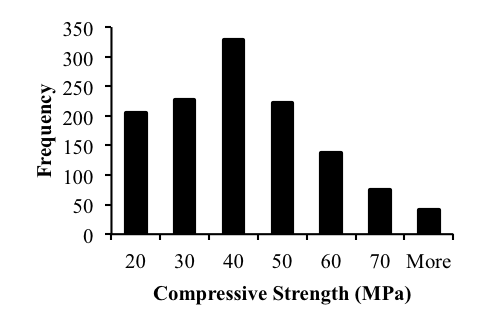
\includegraphics[width=42mm]{data2.png}}
% \subfigure[Caption3]{\label{fig63}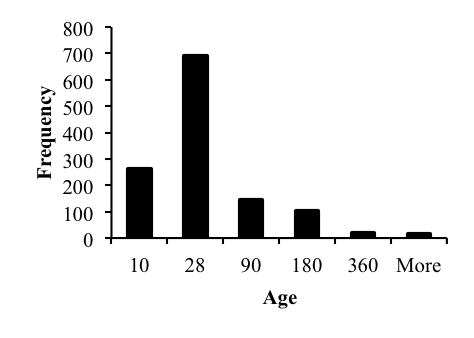
\includegraphics[width=42mm]{data3.png}}
% \caption{Figures sample}
% \end{figure}
% You can add lists into the text like this. 
% \begin{itemize}
% \settowidth{\leftmargin}{{\Large$\square$}}\advance\leftmargin\labelsep
% \itemsep3pt\relax
% \renewcommand\labelitemi{{\lower1pt\hbox{\small$\square$}}}
% \item	Some sample text item 1. 
% \item You may refer to tables \ref{tab1} 
% \item Or figures \ref{fig61}
% \end{itemize}

% Tables can be added like this
% \begin{table}[!htbp]
% \centering
% \caption{Sample table}
% \label{tab1}
% \begin{tabular}{llll}

% \hline
% Column 1 & Column 2 & Column 3       \\\hline
% 1         & Data1 & 13.41179 & 0.9492839 \\
% 2            & Data2 & 13.39824 & 0.9492952\\\hline
% \end{tabular}
% \end{table}


